\chapter{Evaluating Curriculum Learning in Software Engineering tasks}
\label{chapter:chap4}
We adopted the most popular discrete scheduler, known as \textit{Baby Step}, where the complexity of the training
data needs to be gradually increasing. Due to this, a reliable metric to split the initial dataset of each task needed to be defined.
This approach distributes the sorted data into buckets, from easy to hard according to the metric, and starts training with the easiest bucket. 
Starting from the easiest bucket, after a fixed number of training epochs or convergence, the subsequent bucket is merged
into the current training subset - main characteristic of \textit{Baby Step} approach.
Finally, once all the buckets are merged and used, the
training process either stops or continues several extra epochs.\\
Note that, at each epoch the scheduler shuffles the current bucket and samples mini-batches for training.\\
\newline
However, before testing curriculum learning approach, we thougth it was strictly necessary reproducing - in the case 
of bug-fixing task - or conducting -  within the framework of the other 2 tasks - the experiment on the modelbase.\\
We worked with a neural network whose configuration is composed by 1-layer bidirectional Encoder, 2-layer Attention 
Decoder both with 256 units, embedding size of 512, and LSTM RNN cells.\\
\newline
In this chapter, we present how we applied Curriculum Learning to some of Software
Engineering tasks, i.e. \textit{bug-fixing}, \textit{code summarization}, and \textit{log generation}
tasks. \\
For each of the tasks considered, the following aspects are described thoroughly:
\begin{itemize}
    \item \textbf{Difficulty Measurer}: a measure to sort the datasets' instances is needed, each task was experimented with a different metric; 
    \item \textbf{Training Scheduler}: sequence of data subsets are presented to the model following a training schedule.
\end{itemize}
TODO: add connection with LSTM forgetting referring to the experiment on one pass\\
%\item \textbf{Dataset characteristics}: the datasets used are composed by a couple, where the first element is the source of the training, while the second is the target;
\newline
The goal of this study is to asses whether Neural Machine Translation, combined with the Curriculum Learning approach, 
can be used for the tasks experimented. In the following section, the design of our study is described in detail.

% ADDITIONS
% need to add information about training on baseline, i.e. in the introduction you must explain that before trying
% to test the CL approach 

The configuration used by the neural network is composed by 1-layer bidirectional Encoder, 
2-layer Attention Decoder both with 256 units, embedding size of 512, 
and LSTM RNN cells. 

\section{Canonical Training}
Before experiment the curriculum learning approach, we reproduced the baseline approaches for each task experimented
that include the conventional technique of randomly ordering the training samples with the aim to investigate how the performance 
of the original models are, compared to the experiment affected by curriculum learning.
\subsection{Bug-fixing}
As for the bug-fixing task, the datasets used to train the NMT model is the union between \textit{small} and \textit{medium} method-level datasets
used by Tufano \textit{et al.} \cite{Tufano2019}. So, we worked with the standard training, evaluation and test set splits of respectively
99.044, 12.381, and 12.380 instances.\\
It is vital to use new data when evaluating a model to prevent the likelihood of overfitting to the 
training set. However, we decided to evaluate our model as we were building it to find the best parameters of 
a model. To evaluate the model while still building and tuning the model, we used the evaluation set. The neural network
was set up to evaluate the model every 1.000 steps. The training was performed for 60k steps as upper bound, 
out of which we considered the best model, early stopping the model before overfitting considering the loss values computed every 1.000 steps.
The best model configuration was then used to run the inference.
Indeed, after the model was trained, it was evaluated on the test set of unseen buggy code. 
Instead of using the classic greeding decoding that selects the output term \(y_i\) with the highest probability, however, we used another decoding
strategy known as Beam Search. 
%[references 2.3.3 michele tufano]. 
The key idea is that the decoding process keeps track of \textit{k}
hypotheses - being \textit{k} the beam size or width.\\
The beam search algorithm selects multiple tokens for a position in a given sequence based on conditional probability. Moreover, the algorithm
can take any number of \textit{N} best alternatives through a hyperparameter known as beam size or width indeed. Conversely to what greedy search does, 
Beam search broad the search to include other words that might fit better apart from the best word for each position in the sequence.
If Greedy search looks at each position in the output sequence in isolation, deciding the word based on highest probability and then moving down to the resto of the sentence,
Beam search also takes the N best output sequences and look at the current preceding words and probabilities compared to the current position that is being decoded in the sequence.\\
We considered the following sizes: 1 - that corresponds to the Greedy Naïve Approach -, 5, 10, 15, 20, 25, 30, 35, 40, 45, 50.

\subsection{Code summarization}
Regarding the task of code summarization, we selected a random sample of 200k instances from a dataset of 2.1 million items.
Also here we considered the canonical division between training, test and evaluation of respectively 200.000, 105.832, and 106.153 instances.
We trained the model on the training set for 20 epochs, that corresponds to 125.000 steps, and we took the best model over the 20 model configuration evaluated after every epoch,
thus using the best checkpoint to run the inference step. This time, to guide the selection of the best configuration, we used the BLEU values computed on the validation set instead of using
the loss function. Conversely, the results are computed on the test set. Indeed, the same way it was done for the previous task, after the training step the model is
evaluated over the test set of unseen functions to generate code summarizations of such methods.\\
The scope of the training here 
was to make the model able to learn how to summarize pieces of code, starting from a sequence of tokenized methods.

\subsection{Log generation}
As well as happened in both the previous task experimented, also in log generation we considered the well-known split between training set, test set, and evaluation set.
The sets in question are - following the same order - of the amount of 106.382, 12.020, and 13.260. The model was trained for 45 epochs, i.e. 149.625 steps, and 
it must be specified that it was evaluated every epoch. The best configuration in this case was guided on an early-stopping criterion based on BLEU values. 
Once the model was trained, it was evaluated against the test set of unseen methods without log statements and messages in order to assess its ability to correctly inject log statements and messages within methods.

\section{Training with Curriculum Learning}

As stated in the Curriculum Learning literature, the training instances need to be ordered based on the curriculum.
Each of the task considered is related to a different curriculum, specifically the datasets were ordered
following 3 different complexity ideas. Since a curriculum approach requires the definition of a \textbf{Difficulty Measurer}
and a \textbf{Training Scheduler}, we defined those for each task. In the following sections details are explained.

\subsection{Bug fixing task}
Based on the entire training dataset at our dispose of couple of buggy-fixed methods, we defined a Difficulty Measurer to divide the dataset
and a Training Scheduler to rule the order in which the instances were given to the model. Since both the source and the target
were tokenized, we thought that computing the number of changes from the buggy version to the fixed one of each method was a quite reliable
way to define the complexity for the type of instances used in this task.\newline

%\noindent\textbf{Dataset Details.} 
%\noindent\begin{minipage}{.45\textwidth}
%\begin{lstlisting}[language=Java, caption={Buggy code},label={lst:buggy1}, mathescape=true, breaklines=true, frame=tlrb]{Name}
%    public void METHOD_1 ( TYPE_1 VAR_1 ) 
%    { VAR_2 . METHOD_2 ( VAR_3 ) ; 
%    ( VAR_4 ) ++ ; METHOD_3 ( ) ; }
%\end{lstlisting}
%\end{minipage}\hfill
%\begin{minipage}{.45\textwidth}
%\begin{lstlisting}[language=Java, caption={Fixed code},label={lst:fixed1}, mathescape=true, breaklines=true, frame=tlrb]{Name}
%    public void METHOD_1 ( TYPE_1 VAR_1 ) 
%    { if ( VAR_2 . METHOD_2 ( VAR_3 ) ) 
%    { ( VAR_4 ) ++ ; METHOD_3 ( ) ; } }
%\end{lstlisting}
%\end{minipage}
%%%%%%%%%%%%%%%%%%%%%%%
% TODO: Insert instance ex.
%%%%%%%%%%%%%%%%%%%%%%%

%%% DATASET DESCRIPTION
\noindent\textbf{Difficulty Measurer.} As stated above, a difficulty measurer definition is the core element of the approch implemented.
For the task at issue here the \textbf{Levenshtain distance} was used as metric. The \textit{Levenshtein distance}, also known as the \textit{edit distance}, 
was introduced by Vladimir Levenshtein in 1965 \cite{Levenshtein_SPD66}. It is a string metric for measuring difference between two sequences, specifically the number of insertions, deletions, and substitutions
required to transform one string into the other. However, the distance we used for our experiments was token based, thus the granularity is word based instead of being single-character based.\\
Defined the measure, the distance between buggy and fixed method for each of the BFPs was computed and we observed the data distribution; then we used the quartiles' values to divide the initial dataset in multiples
smaller datasets, where each of these represents a different level of difficulty.\\
By doing so, we clearly obtained 4 level of difficulty; thus we defined an incremental difficulty criteria to feed the model with: 
the bug-fixing training scheduler described as follows.\newline

%%%%%%%%%%%%%%%%%%%%%%%
% TODO: Insert data distribution figure
%%%%%%%%%%%%%%%%%%%%%%%

\noindent\textbf{Training Scheduler.} The training scheduler decides the sequence of data subsets throughout the training process based
on the judgment from the difficulty measurer. As mentioned in the introduction of this chapter, Baby Step approach switches to the next difficulty level
as soon as the model converges on the previous one.
In the bug-fixing task, the scheduler adjusts
the training data subsets based on an early stopping criterion: after a fixed number of steps
early stopping is run and it considers the model as being converging if the loss value
does not improve after 5K steps.


\subsection{Code summarization task}
As well as happened for the training on the baseline model, a random sample of 200K method-comment pairs was picked from the initial dataset;
evaluation and test datasets, however, were used as-is. This initial dataset was then divided in 4 sub-datasets, each representing a different
level of difficulty.\newline  

%\begin{lstlisting}[language=Java, caption={Function},label={lst:buggy1}, mathescape=true, breaklines=true]{Name}
%    protected String creatorName() {
%        return Texts.getText("solver");
%    }
%\end{lstlisting}

%\begin{lstlisting}[language=Java, caption={Comment},label={lst:fixed1}, mathescape=true, breaklines=true]{Name}
%    //Gives the name of this solver as used to tag new solutions.
%    //@return the name of this solver
%\end{lstlisting}


%%%%%%%%%%%%%%%%%%%%%%%
% TODO: Insert instance ex.
%%%%%%%%%%%%%%%%%%%%%%%

\noindent\textbf{Difficulty Measurer.} In Natural Language Processing tasks, the \textbf{sentence lenght} intuitively expresses the complexity 
of a sentence, thus we used the instances' lenghts as measure of complexity. 
However, instead of focusing on the source of the couple, for this task we decided to sort out the subdatasets computing the
difficulty measure on the target, namely the lenght of each method's comment. 
Once obtained the lenghts, accordingly to the data distribution we took advantage of the quartiles obtained to split the intial dataset in 4 smaller 
buckets. 
\begin{figure}[h!]
    \begin{center}
        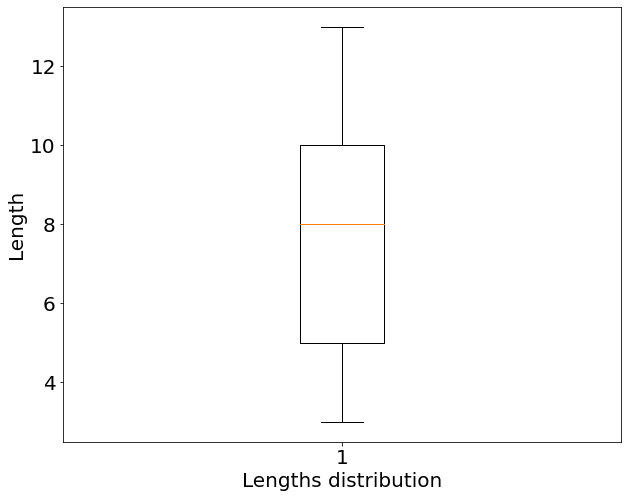
\includegraphics[width=0.35\textwidth]{/Users/carmenarmenti/Desktop/Thesis document/images/boxplot-length.png}
        \caption{\label{fig:CSdistribution}Code summarization task: data distribution.}
    \end{center}
\end{figure}
%%%%%%%%%%%%%%%%%%%%%%%
% TODO: Insert data distribution figure
%%%%%%%%%%%%%%%%%%%%%%%
Accordingly to the training set, the evaluation set was splitted in 4 sub-datasets as well, because the model trained on a defined level (or levels) of difficulty
needs to be evaluated on instances with the same complexity, according to the curriculum learning idea.\newline

\noindent\textbf{Training Scheduler.} Similarly to what happens in bug-fixing task, the training scheduler decides to sample from more harder data only when the model converges on the 
previous easier bucket. The convergence is assessed after a fixed number of epochs, after which early stopping with patience of 5 epochs
is run. Once the model converges on the first bucket, the training proceeds on the second and so forth. 

\subsection{Log generation task}
Inserting log messages is a practice broadly used and decide where to inject log statements, what information to report through it, 
and at which log level is as hard as it is crucial \cite{Mastropaolo2022}. In the following section Curriculum Learning approach 
is applied at log generation task. The dataset for this task is composed by couple of methods, where the source is the method without the log statement,
the target instead has not only the log statement but also the log message.\\
Those couples where used to train the model to generate and inject log statements in Java code.
If the training set for the training on the baseline model was composed by 106.382, the training set for the experiment with curriculum learning 
is of 105.985 instances. This was because of the Difficulty Measurer we choose to use: according to the latter, 397 instances had a null difficulty, hence
were excluded from the set. The same happend in the case of the evaluation set, 13.197 instances were used instead of 13.260. 
The test set ??? \newline


%\noindent\begin{minipage}{.45\textwidth}
%\begin{lstlisting}[language=Java, caption={Method},label={lst:buggy1}, mathescape=true, breaklines=true]{Name}
%    public CsvDestination setPath ( final String path ) 
%    { if ( csvFile != null ) 
%    { throw new UnsupportedOperationException ( ""Changing the value of path after opening the destination is not allowed."" ) ; } 
%    if ( outputChannel != null ) 
%    { try 
%    { outputChannel . close ( ) ; 
%    outputChannel = null ; } 
%    catch ( final IOException e ) { } } 
%    this . path = path ; 
%    return this ; }
%\end{lstlisting}
%\end{minipage}\hfill
%\begin{minipage}{.45\textwidth}
%\begin{lstlisting}[language=Java, caption={Method + log statement},label={lst:fixed1}, mathescape=true, breaklines=true]{Name}
%    public CsvDestination setPath ( final String path ) 
%    { if ( csvFile != null ) 
%    { throw new UnsupportedOperationException ( ""Changing the value of path after opening the destination is not allowed."" ) ; } 
%    if ( outputChannel != null ) 
%    { try 
%    { outputChannel . close ( ) ; 
%    outputChannel = null ; } 
%    catch ( final IOException e ) 
%    { log . error ( String . format ( ""Could not close file channel with CSV results for file %s."" , csvFile ) , e ) ; } } 
%    this . path = path ; 
%    return this ; }
%\end{lstlisting}
%\end{minipage}

%%%%%%%%%%%%%%%%%%%%%%%
% TODO: Insert instance ex.
%%%%%%%%%%%%%%%%%%%%%%%

\noindent\textbf{Difficulty Measurer.} Given the dataset at our dispose we choose as difficulty measurer the 
complexity of the instruction set in program execution tasks. More specifically we 
computed \textbf{cyclomatic complexity} through Lizard tool \cite{lizard}. Cyclomatic complexity
is a quantitative software metric developed by Thomas J. McCabe in 1976, used to indicate
the complexity of a program.  
It measures the number of linearly-independent paths through a program module. 
The measure is computed using the control-flow graph of the program where
the nodes of the graph correspond to sets of commands of a program, and
a directed edge connects 2 nodes if the second command might be executed
immediately after the first command. It can be applied to individual functions,
modules, methods or classes within a program. We decided to compute it on each of
the source methods.\\
It must be said that from the initial dataset were removed 397 instances whose
cyclomatic complexity was 0. Decided and computed the difficulty measure
for each instance, the dataset was ready to be used by the training scheduler.\newline

%%%%%%%%%%%%%%%%%%%%%%%
% TODO: Insert data distribution figure
%%%%%%%%%%%%%%%%%%%%%%%

\noindent\textbf{Training Scheduler.} Once again we observed the data distribution and considered the 3 quartiles
to divide the whole dataset in 4 subsets. Each of those represented a different level of difficulty.\\
As soon as the model converged on the current bucket, BLEU values after each epoch were assessed,
and early stopping was applied. We took the best model before divergence to restart the training 
from the following bucket. 


%%%%%%%%%%%%%%%%%%%%%%%
%RANDOM NOTES: 
%to use to sort the instances at dispose
%Only after this choice the initial dataset
%was divided in multiple smaller datasets For the task at issue here 
%the instances of th

%Once defined the measure, we were able to divide the initial dataset in smaller datasets so as to define 
%an incremental difficulty criteria to feed the model with. 

%For each of the task considered, a different metric to split the datasets was used.
%%%%%%%%%%%%%%%%%%%%%%%




